This project's aim was to develop the theoretical landscape of equivariant GNN architectures. For this reason, synthetic tests of \textit{expressivity} were chosen over performance benchmarking as this would better show the contributions of the CMACE architecture. Expressivity is a measure of the range and complexity of functions that an architecture can approximate. For example, the linear regression model $y = \alpha x + \beta$ is not expressive enough to approximate the function $y = x^2$. However, note that expressivity is a subjective measure highly dependent on the kind of task you are measuring against. For example, an architecture that is extremely capable in one domain but cannot complete a trivial task in another. Therefore choosing the right measures of expressivity is of the utmost importance. 

\begin{figure}[H]
    \centering
    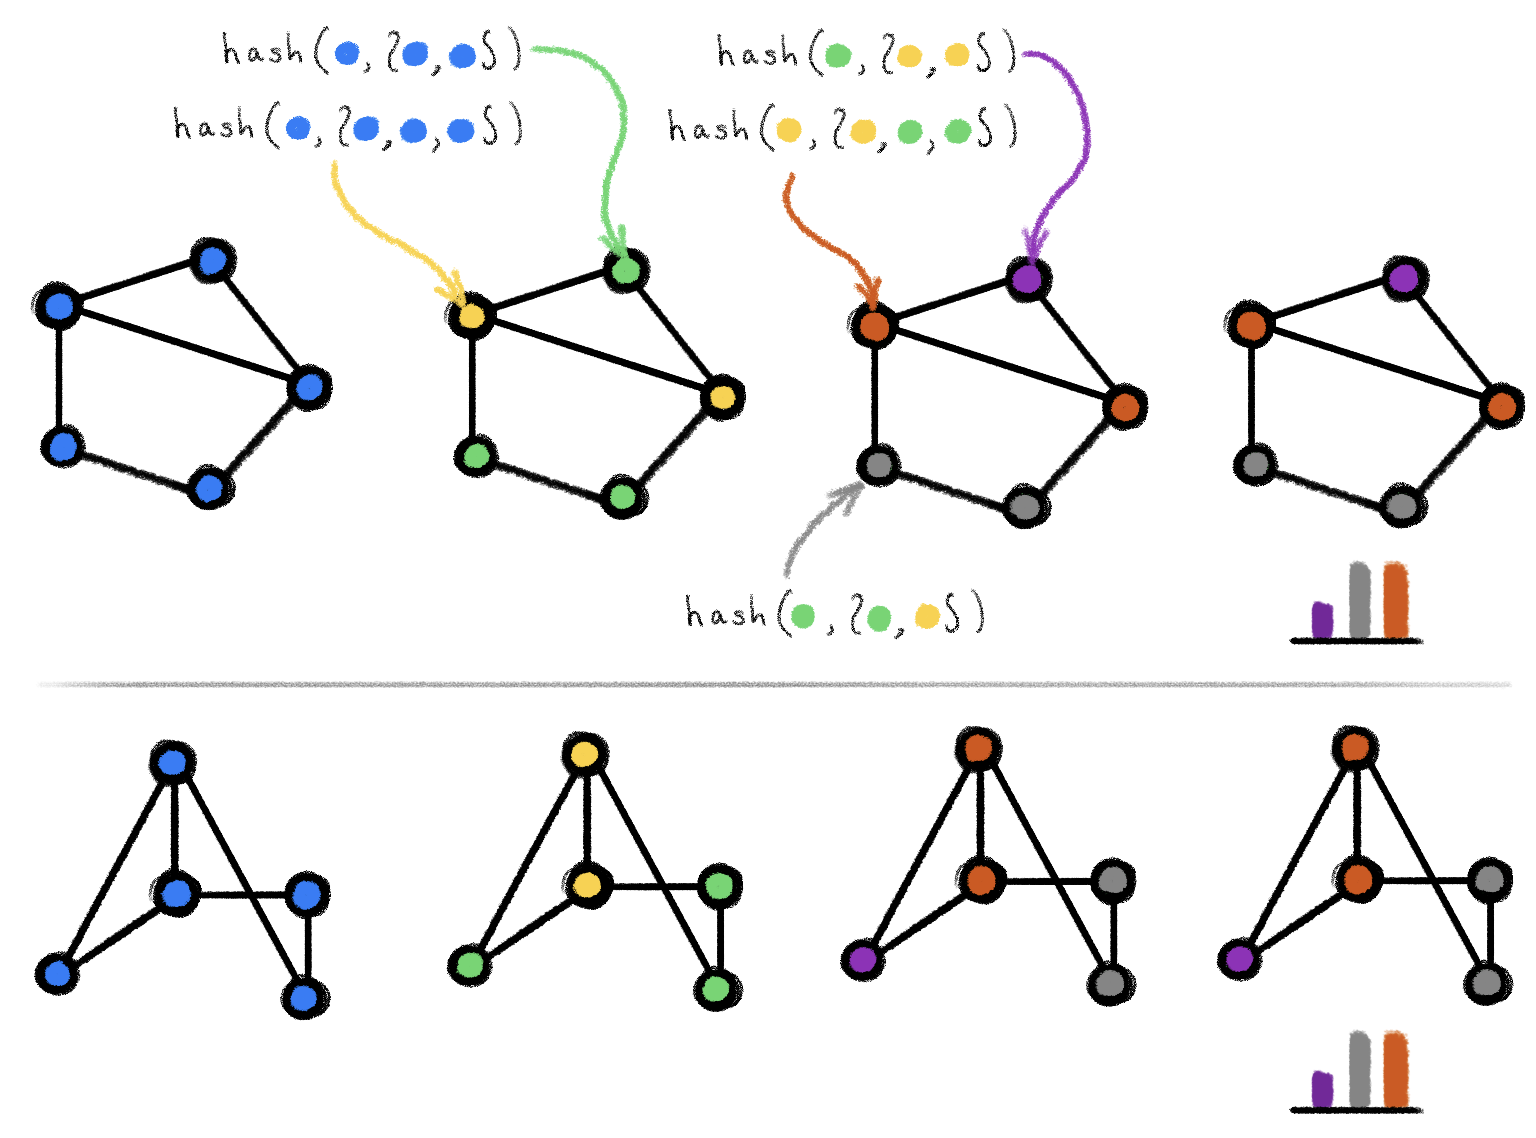
\includegraphics[scale=0.2]{figures/wl-test.png}
    \caption{WL test for two graphs, which here, are isomorphic and thus have the same proportions of colours at the end  \cite{Bronstein2020}}
    \label{fig:wl-test}
\end{figure}

When thinking about such tests for equivariant GNNs we ought to look at non-trivial problems on graphs - one classical example is a test for graph isomorphism. This is an enticing property for GNNs to have - if a graph doesn't have this property it will represent non-identical graphs in the same way which leaves us little place to classify aspects of them differently. The algorithm to solve this problem \cite{read1977graph} is the Weisfeiler-Lehman (WL) test \cite{weisfeiler1968reduction}. To see how the WL works, it is easiest to look at the example in Figure \ref{fig:wl-test}. 

Initially, all nodes are given the same `colour'. The current colour of a node and the multiset created by aggregating the colours of neighbouring nodes is used as an input to an one-to-one hash function which provides a new colour. Then repeat the process until the colouring is stable. If the stable colouring of two graphs is different then the graphs are not isomorphic. If the colouring of two graphs is the same they have met a necessary (but not sufficient) condition of isomorphism. The WL test is very reminiscent of message passing as the central node aggregates features of its neighbours, except in this process the propagation of information is lossless due to the fact that the hash function is one-to-one. With this perspective as the WL test as a perfect GNN testing for isomorphism, it is unsurprising that it has been shown that GNNs are at best as good the WL for isomorphism testing \cite{xu2018powerful}.

\begin{figure}[H]
    \centering
    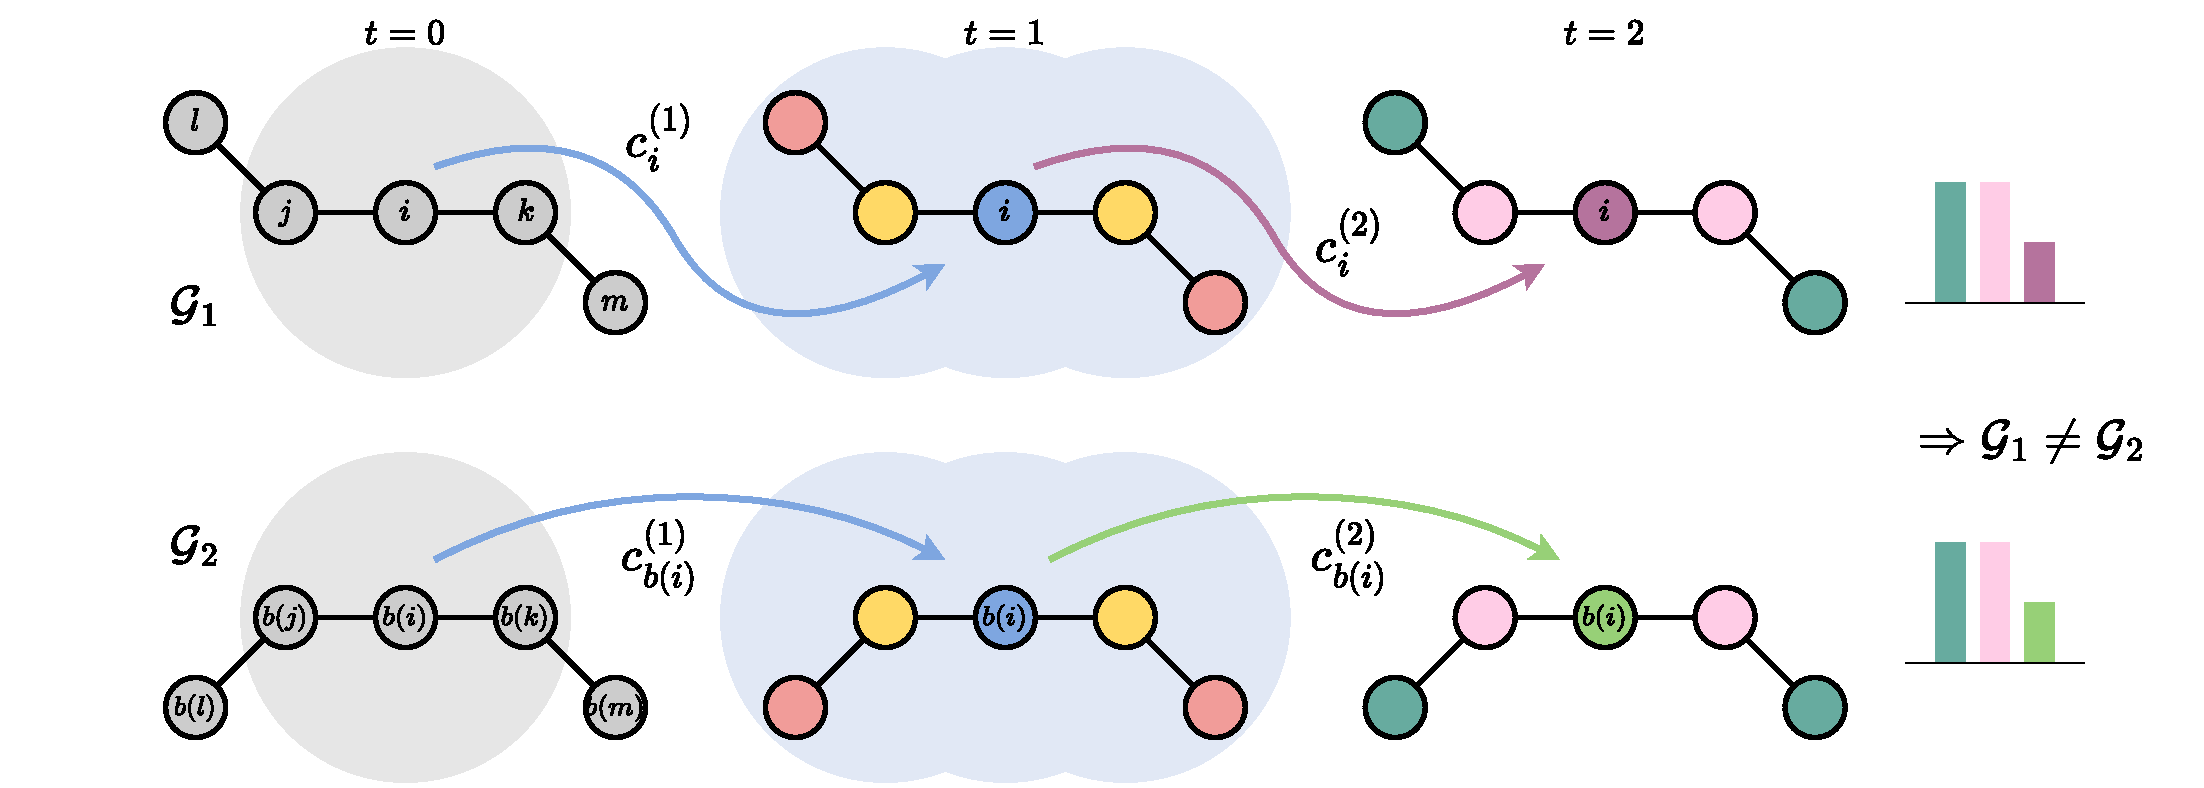
\includegraphics[width=\textwidth]{figures/gwl.pdf}
    \caption{Geometric WL test for two graphs that are non-isomorphic once geometry is considered. Here, geometric information about the angles on the ends to the middle, once these equivariants `meet' in the middle, the two graphs can be seen to be different by the GWL test \cite{joshi2023expressive}. This new found way of telling graphs apart motivates GWL}
    \label{fig:gwl}
\end{figure}

For Geometric GNNs the notion of isomorphism is stricter as the relative positions also have to be the same in addition to the graph structure. This required the creation of the Geometric WL (GWL) test \cite{joshi2023expressive} which like its analogue is shown as the upper bound for geometric graph isomorphism testing. Therefore, it is worth using the GWL as a baseline measure of expressivity. The action of GWL is shown in Figure \ref{fig:gwl} and will be used in the second of our experiments. Both experiments are from the testing environment in the \texttt{geometric-gnn-dojo}\footnote{Code available on GitHub: \url{https://github.com/chaitjo/geometric-gnn-dojo}}.

\subsection{Rotational symmetry}

\begin{table}[H]
    \centering
    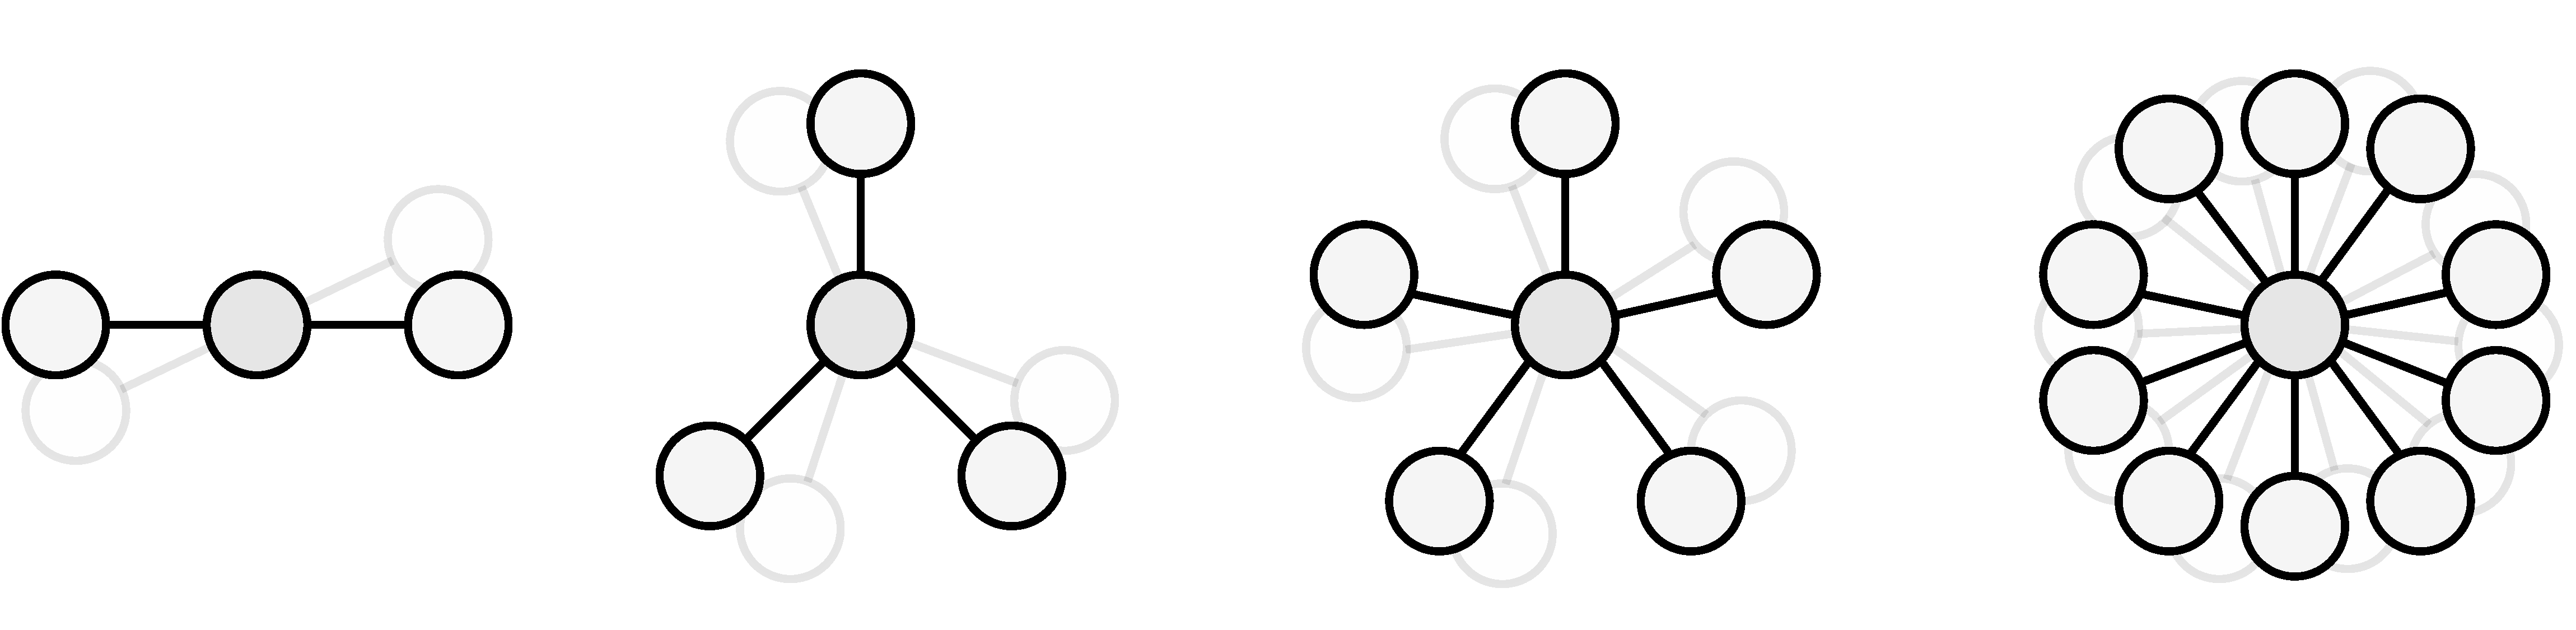
\includegraphics[width=0.6\linewidth]{figures/rotsym.pdf}
     \resizebox{0.8\linewidth}{!}{
    \begin{tabular}{clcccc}
        \toprule
        & & \multicolumn{4}{c}{\textbf{Rotational symmetry}} \\
        & \textbf{GNN Layer} & 2 fold & 3 fold & 5 fold & 10 fold \\
        \midrule
        \multirow{7}{*}{\rotatebox[origin=c]{90}{Cartesian}} 
        & E-GNN$_{L=1}$ & \cellcolor{red!10} 50.0 ± 0.0 & 50.0 ± 0.0 & 50.0 ± 0.0 & 50.0 ± 0.0 \\
        & GVP-GNN$_{L=1}$ & \cellcolor{red!10} 50.0 ± 0.0 & 50.0 ± 0.0 & 50.0 ± 0.0 & 50.0 ± 0.0 \\ 
        & CMACE$_{L=1}$ & \cellcolor{red!10} 50.0 ± 0.0 & 50.0 ± 0.0 & 50.0 ± 0.0 & 50.0 ± 0.0 \\
        & CMACE$_{L=2}$ & \cellcolor{green!10} \textbf{100.0 ± 0.0} & 50.0 ± 0.0 & 50.0 ± 0.0 & 50.0 ± 0.0 \\
        & CMACE$_{L=3}$ & \cellcolor{green!10} \textbf{100.0 ± 0.0} & \cellcolor{green!10} \textbf{100.0 ± 0.0} & 50.0 ± 0.0 & 50.0 ± 0.0 \\
        & CMACE$_{L=5}$ & \cellcolor{green!10} \textbf{100.0 ± 0.0} & \cellcolor{green!10} \textbf{100.0 ± 0.0} & \cellcolor{green!10} \textbf{100.0 ± 0.0} & 50.0 ± 0.0 \\
        & CMACE$_{L=10}$ & \cellcolor{green!10} \textbf{100.0 ± 0.0} & \cellcolor{green!10} \textbf{100.0 ± 0.0} & \cellcolor{green!10} \textbf{100.0 ± 0.0} & \cellcolor{green!10} \textbf{100.0 ± 0.0} \\
        \midrule
        \multirow{5}{*}{\rotatebox[origin=c]{90}{Spherical}}
        & TFN/MACE$_{L=1}$ & \cellcolor{red!10} 50.0 ± 0.0 & 50.0 ± 0.0 & 50.0 ± 0.0 & 50.0 ± 0.0 \\
        & TFN/MACE$_{L=2}$ & \cellcolor{green!10} \textbf{100.0 ± 0.0} & 50.0 ± 0.0 & 50.0 ± 0.0 & 50.0 ± 0.0 \\
        & TFN/MACE$_{L=3}$ & \cellcolor{green!10} \textbf{100.0 ± 0.0} & \cellcolor{green!10} \textbf{100.0 ± 0.0} & 50.0 ± 0.0 & 50.0 ± 0.0 \\
        & TFN/MACE$_{L=5}$ & \cellcolor{green!10} \textbf{100.0 ± 0.0} & \cellcolor{green!10} \textbf{100.0 ± 0.0} & \cellcolor{green!10} \textbf{100.0 ± 0.0} & 50.0 ± 0.0 \\
        & TFN/MACE$_{L=10}$ & \cellcolor{green!10} \textbf{100.0 ± 0.0} & \cellcolor{green!10} \textbf{100.0 ± 0.0} & \cellcolor{green!10} \textbf{100.0 ± 0.0} & \cellcolor{green!10} \textbf{100.0 ± 0.0} \\
        \bottomrule
    \end{tabular}  
    }
    \caption{\textit{Rotationally symmetric structures.} Here expressive power is probed via training single layers of equivariant GNNs to tell apart an $L$-fold symmetric with have been rotated about the axis of symmetry. Previous work has shown that layers using tensors of rank-$L$ are unable to differentiate between the rotated versions of graphs with greater than $L$-fold symmetry \cite{joshi2023expressive}. This experiment shows \textbf{CMACE is as powerful as MACE at telling apart rotationally symmetric environments}. Data from non-CMACE models and table adapted from Joshi et al. 2023 \cite{joshi2023expressive}. Anomolous results are marked in \colorbox{red!10}{red} and expected results in \colorbox{green!10}{green}.
    }
    \label{tab:rotsym}
\end{table}

This first task investigates how well different models could detect differences in rotationally symmetric environments that are orientated differently. This is useful as neighbourhoods like this appear very often in the material sciences in periodic structure. 

\textbf{Experiment. } First, a graph with $L$-fold symmetry is created (a central node with $L$ equally space spokes), and a second graph is created by rotating the first graph at an angle, $0 < \theta < \frac {2\pi} L$ about the central node (see examples in Figure on top of Table \ref{tab:rotsym}). Both graphs are then fed into the model, if it can tell the two graphs apart (i.e. has two different outputs) then the graph is expressive enough to detect this $L$-fold symmetry. The test is run on pairs of graphs with $L=2,3,5,10$.

\textbf{Results. } It has been previously shown empirically, a model using tensors with a maximum rank $L$ is unable to tell apart the graph pairs described above for rotational symmetries greater than $L$-fold \cite{joshi2023expressive}. As expected, CMACE models with maximum rank tensors of varying $L$ exhibited the same behaviour as TFN/MACE becoming the first Cartesian model to have the expressive power to tell apart these kinds of neighbourhoods.

\subsection{$k$-chains}

\begin{table}[H]
    \centering
    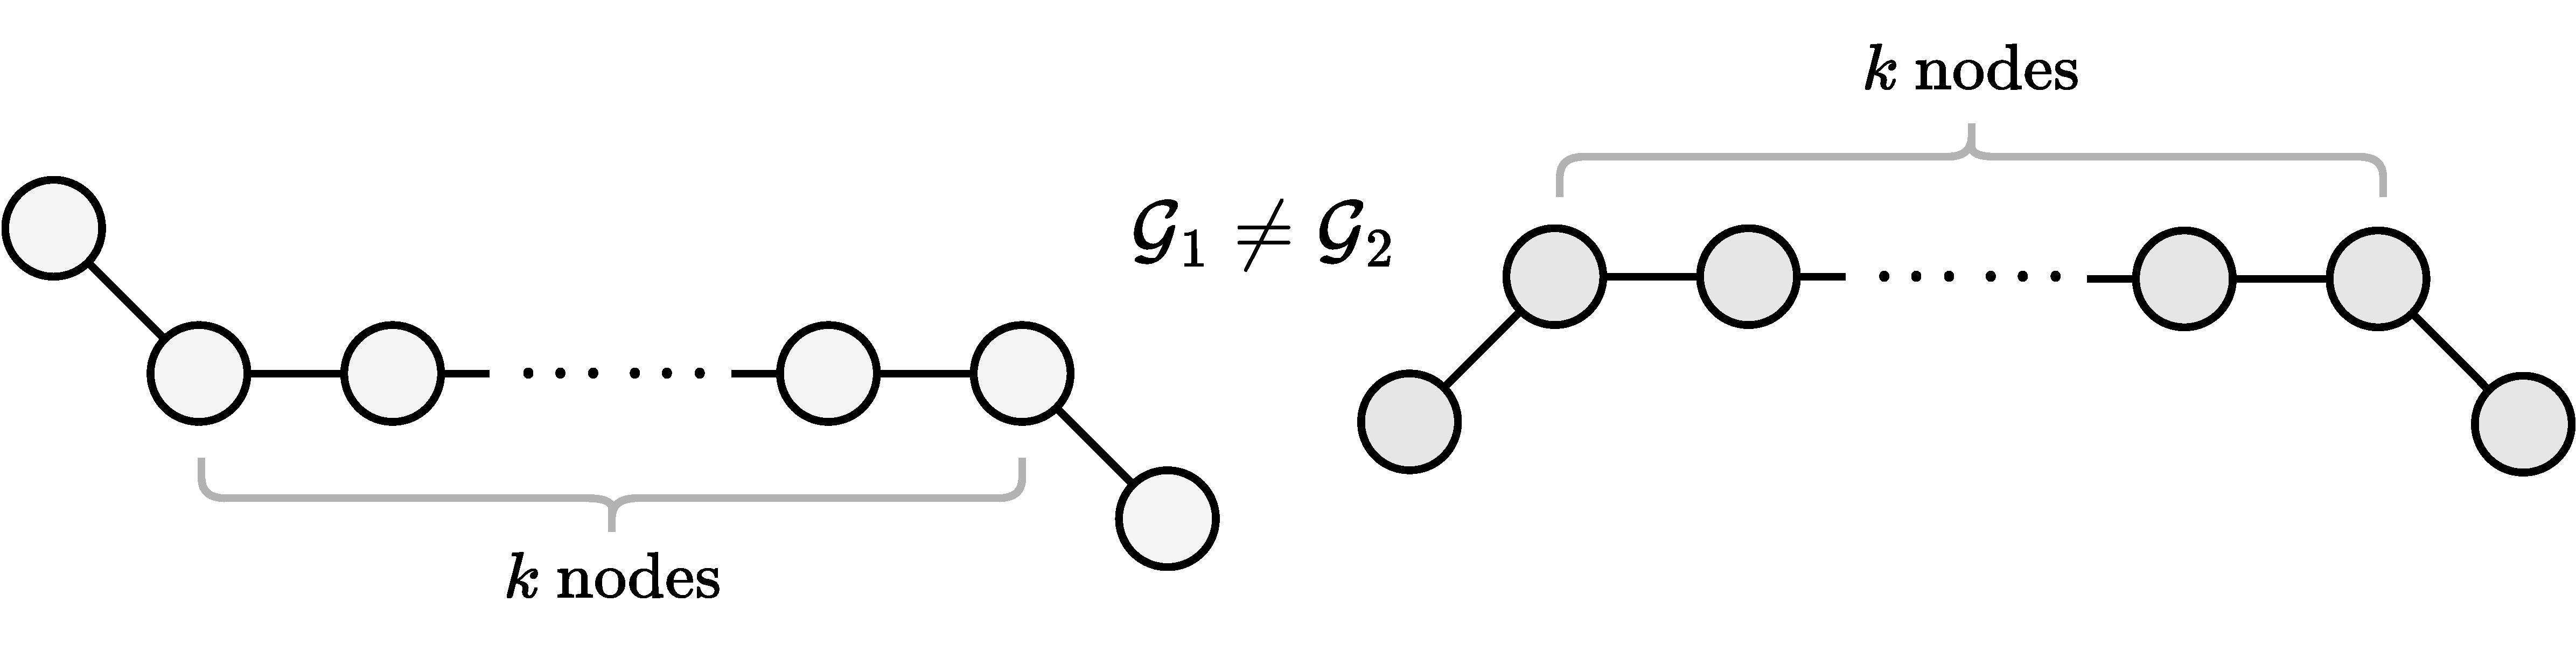
\includegraphics[width=0.6\linewidth]{figures/kchains.pdf}
    \resizebox{0.9\linewidth}{!}{
    \begin{tabular}{clccccc}
        \toprule
        & ($k=\mathbf{4}$-chains) & \multicolumn{5}{c}{\textbf{Number of layers}} \\
        & \textbf{GNN Layer} & $\lfloor \frac{k}{2} \rfloor$ & \cellcolor{gray!10} $\lfloor \frac{k}{2} \rfloor + 1 = \mathbf{3}$ & $\lfloor \frac{k}{2} \rfloor + 2$ & $\lfloor \frac{k}{2} \rfloor + 3$ & $\lfloor \frac{k}{2} \rfloor + 4$ \\
        \midrule
        \multirow{3}{*}{\rotatebox[origin=c]{90}{Inv.}} &
        \gray{IGWL} & \gray{50\%} & \gray{50\%} & \gray{50\%} & \gray{50\%} & \gray{50\%} \\
        & SchNet & 50.0 ± 0.00 & 50.0 ± 0.00 & 50.0 ± 0.00 & 50.0 ± 0.00 & 50.0 ± 0.00 \\
        & DimeNet & 50.0 ± 0.00 & 50.0 ± 0.00 & 50.0 ± 0.00 & 50.0 ± 0.00 & 50.0 ± 0.00 \\
        \midrule
        \multirow{5}{*}{\rotatebox[origin=c]{90}{Equiv.}} &
        \gray{GWL} & \gray{50\%} & \gray{\textbf{100\%}} & \gray{\textbf{100\%}} & \gray{\textbf{100\%}} & \gray{\textbf{100\%}} \\
        & E-GNN & 50.0 ± 0.0 & \cellcolor{red!10} 50.0 ± 0.0 & \cellcolor{red!10} 50.0 ± 0.0 & \cellcolor{red!10} 50.0 ± 0.0 & \cellcolor{green!10} \textbf{100.0 ± 0.0} \\
        & GVP-GNN & 50.0 ± 0.0 & \cellcolor{green!10} \textbf{100.0 ± 0.0} & \cellcolor{green!10} \textbf{100.0 ± 0.0} & \cellcolor{green!10} \textbf{100.0 ± 0.0} & \cellcolor{green!10} \textbf{100.0 ± 0.0} \\
        & TFN & 50.0 ± 0.0 & \cellcolor{red!10} 50.0 ± 0.0 & \cellcolor{red!10} 50.0 ± 0.0 & \cellcolor{green!10} \textbf{80.0 ± 24.5} & \cellcolor{green!10} \textbf{85.0 ± 22.9} \\
        & MACE & 50.0 ± 0.0 & \cellcolor{green!10} \textbf{90.0 ± 20.0} & \cellcolor{green!10} \textbf{90.0 ± 20.0} & \cellcolor{green!10} \textbf{95.0 ± 15.0} & \cellcolor{green!10} \textbf{95.0 ± 15.0} \\
        & CMACE & 50.0 ± 0.0 & \cellcolor{green!10} \textbf{95.0 ± 15.0} & \cellcolor{green!10} \textbf{90.0 ± 20.0} & \cellcolor{green!10} \textbf{90.0 ± 20.0} & \cellcolor{green!10} \textbf{80.0 ± 24.5} \\
        \bottomrule
    \end{tabular}
    }
    \caption{\textit{$k$-chain geometric graphs.} This experiment investigates \textbf{how well different architectures propagate geometric information}, where the GWL test is an upper bound, propagating information perfectly. According to the GWL test, the $k$-chains graphs are ($\lfloor \frac k 2 \rfloor +1$)-layer distinguishable, as it takes this long for the geometric information from both ends to meet in the middle. We train models with a varying number of layers for $k=4$ and find that \textbf{like MACE, CMACE can faithfully propagate geometric information most of the time}, but sometimes struggles with bottle-necking. Data from non-CMACE models and table adapted from Joshi et al. 2023 \cite{joshi2023expressive}.
    }
    
    \label{tab:kchains}
\end{table}

\textbf{Experiment.} The $k$-chains experiment is a generalisation of previous analysis of equivariant models \cite{schutt2021equivariant}. The aim is to investigate how well (if at all) architectures propagate geometric information across the graph during multiple message-passing steps (i.e. multiple layers). As discussed earlier GWL propagates this information perfectly, without loss therefore this experiment is a test of how close our model is to geometric information propagation. The synthetic data was made from graphs that have a straight chain of $k$ nodes and then have two nodes on each end that can either point at an angle $\frac \pi 4$ upwards or downwards. For one graph, both end nodes point downwards and in the other one points down, and the other points up (see schematic at top of Table \ref{tab:kchains} and Figure \ref{fig:gwl}). 

Figure \ref{fig:gwl} shows GWL (i.e. perfect propagation) on a pair of graphs for $k=3$. After one layer ($t=1$), both have the same colour, therefore these graphs appear the same after one layer. Whereas, after two layers, due the geometric from both ends mixing the middle nodes node gives a different colour for the two different graphs. After each layer, the information from a node is taken into account for the colour of the neighbouring nodes in the next layer, only when the information about the end nodes mixes in the middle do we get different results as they ends have different relative values in graph 1 vs graph 2. Therefore, at best, it takes $\lfloor \frac k 2 \rfloor + 1$ layers (floor function to account for even and odd $k$) for the geometric information about the two end nodes to mix causing the model to achieve different values.

\textbf{Results. } We used $k=4$ to match the implementation of the paper where this test first appeared. As expected, when using fewer than $\lfloor \frac k 2 \rfloor + 1$ layers, our model couldn't tell apart the two graphs at all. When using more than the required number of layers, the performance shows that most of the time it was possible to tell them apart although sometimes our model could not, this shows how our model is not a perfect GNN i.e. GWL performance is 100\% when greater than minimum number of layers. This pathology is caused by bottle-necking, i.e. the bandwidth of the single path to the central node is not big enough to faithfully propagate the geometric information. These results were only comparable to MACE showing we have the same property of good but sometimes limited propagation of geometric information. 


